%!TEX TS-program = lualatex
%!TEX encoding = UTF-8 Unicode

\documentclass[t]{beamer}

%%%% HANDOUTS For online Uncomment the following four lines for handout
%\documentclass[t,handout]{beamer}  %Use this for handouts.
%\includeonlylecture{student}
%\usepackage{handoutWithNotes}
%\pgfpagesuselayout{3 on 1 with notes}[letterpaper,border shrink=5mm]

%%% Including only some slides for students.
%%% Uncomment the following line. For the slides,
%%% use the labels shown below the command.

%% For students, use \lecture{student}{student}
%% For mine, use \lecture{instructor}{instructor}


%\usepackage{pgf,pgfpages}
%\pgfpagesuselayout{4 on 1}[letterpaper,border shrink=5mm]

% FONTS
\usepackage{fontspec}
\def\mainfont{Linux Biolinum O}
%\setmainfont[Ligatures={Common,TeX}, Contextuals={NoAlternate}, BoldFont={* Bold}, ItalicFont={* Italic}, Numbers={OldStyle}]{\mainfont}
\setsansfont[Scale=MatchLowercase, Numbers={Lining}, Ligatures={Common, TeX}]{\mainfont} 
\newfontface\liningnums[Numbers=Lining, Scale=MatchLowercase]{\mainfont}

%\usepackage{microtype}


%\addfontfeatures{Numbers=SlashedZero}

\usepackage{graphicx}
	\graphicspath{%
	{/Users/mtaylor/Pictures/teach/434/lectures/}%
	{/Users/mtaylor/Pictures/teach/348/lectures/}%
	{/Users/mtaylor/Pictures/teach/434/handouts/}%
	{/Users/mtaylor/Pictures/teach/common/}%}%
	{img/}} % set of paths to search for images

\usepackage{xcolor}

%\usepackage{amsmath,amssymb}

%\usepackage{units}

%\usepackage{siunitx}
\usepackage{booktabs}
\usepackage{multicol}
%	\setlength{\columnsep=1em}

\usepackage{array}
\newcolumntype{L}[1]{>{\raggedright\let\newline\\\arraybackslash\hspace{0pt}}p{#1}}
\newcolumntype{C}[1]{>{\centering\let\newline\\\arraybackslash\hspace{0pt}}p{#1}}
\newcolumntype{R}[1]{>{\raggedleft\let\newline\\\arraybackslash\hspace{0pt}}p{#1}}

%\usepackage{chemfig}
\usepackage[version=4]{mhchem}

\usepackage{tikz}
	\tikzstyle{every picture}+=[remember picture,overlay]
	\usetikzlibrary{arrows,calc}

\mode<presentation>
{
  \usetheme{Lecture}
  \setbeamercovered{invisible}
  \setbeamertemplate{items}[default]
}

%\usepackage{hyperref}


\usepackage{calc} % Necessary for hidden word function.
\newcommand\HiddenWord[1]{%
	\alt<handout>{\rule{\widthof{#1}}{\fboxrule}}{#1}%
}

% Use the to temporarily set a background grid for positioning.
%\setbeamertemplate{background}[grid][step=1em]


\begin{document}

\lecture{student}{student}

{
\usebackgroundtemplate{\includegraphics[width=\paperwidth]{14_climate_change_impacts}}
\begin{frame}[b]{Climate change affects many oceanic processes.}

	\tiny Fig.~19.1 \copyright\,Sinauer Associates, Inc.
\end{frame}
}
%
\begin{frame}{About 25\% of \ce{CO2} released since the Industrial Revolution is sequestered in the oceans.}

	\includegraphics[width=\textwidth]{14_industrial_revolution}
	
	\vfilll \tiny D.\,W.\,F.~Hardie, Wikimedia, public domain
	
	
\end{frame}
%
\begin{frame}[t]{Accumulation of atmospheric \ce{CO2} causes ocean acidification.}

	\includegraphics[width=\textwidth]{14_mauna_loa_co2}
	
	\vfilll

	\hfill \tiny Fig.~19.3 \copyright\,Sinauer Associates, Inc.
	
\end{frame}
%
%\begin{frame}[t]{Global temperatures were relatively steady until recently.}
%
%	{\centering
%		\includegraphics[height=0.82\textheight]{14_historic_temperatures}\par
%	}
%	
%	\vfilll
%	
%	\hfill \tiny Mann et al. 2008. PNAS 105: 13252.  
%	
%\end{frame}
%%
%\begin{frame}[t]{Global temperatures are increasing rapidly.}
%
%	\includegraphics[width=\textwidth]{14_historic_temperature_change_rate}
%
%	\vfilll
%	
%	\hfill \tiny Tamino 2013, modified Shakun et al. 2012, Marcott et al. 2013
%
%\end{frame}
%%

\begin{frame}[t]{Holocene \ce{CO2} and pH will change rapidly.}

	\includegraphics[width=\textwidth]{14_holocene_co2_ph}
	
	\vfilll
	
	\hfill \tiny \href{https://www.nature.com/scitable/knowledge/library/ocean-acidification-25822734}{Nature.com/scitable: Ocean Acidification}

\end{frame}
%
\begin{frame}[t]{How does the predicted future compare to the past for \ce{CO2} and pH?}

	{\centering\liningnums\begin{tabular}{@{}L{25mm}C{20mm}C{10mm}R{25mm}@{}}
		\toprule
		Time	&	p\ce{CO2}\newline (seawater) &	pH	&	[\ce{H+}] Increase (pre-industrial) \\
		\midrule
		Glacial	&	180	& 8.32	&	$-$30.8\% \\[1ex]
		Pre-Industrial	&	280	&	8.16	&	— \\[1ex]
		Present	&	380	&	8.05	&	$+$28.9\% \\[1ex]
		2 $\times$ \ce{CO2} (pre-industrial)	&	560	&	7.91	&	$+$77.7\% \\[1ex]
		3 $\times$ \ce{CO2} (pre-industrial) & 	840	& 7.76 & $+$151.4\% \\[1ex]
		\bottomrule
	\end{tabular}\par
	}

	\hangpara \highlight{Current atmospheric \ce{CO2} is sustained above 400 ppm!} 
	\vfilll

	\hfill \tiny Kleypas et al. 2006. NOAA Workshop Report.

\end{frame}
%
\begin{frame}[t]{pH is maintained by the \highlight{bicarbonate buffering system.}}

	\includegraphics[width=0.98\textwidth]{14_carbonate_buffering_ratios_no_change}
	
	\begin{tikzpicture}
		\draw [blue] (20.9em,5.3em) -- node [right] {Current pH} (20.9em,20.2em);
	\end{tikzpicture}

	\vfilll
	
	\hfill \tiny BeAr, Wikimedia, public domain
\end{frame}
%
\begin{frame}[t]{Atmospheric [\ce{CO2}] determines ocean pH.}

	{\centering \ce{CO2 + H2O <-> H2CO3 <-> H+ + HCO3- <-> 2H+ + CO3^{2-}}\par
	}

	\vspace*{2\baselineskip}

	\hspace*{1em}\begin{tabular}{@{}ll@{}}
	[\ce{HCO3^-}] &	\textasciitilde90\% inorganic carbon \\[1em]
	[\ce{CO3^2-}] &	 \textasciitilde9\% inorganic carbon\\[1em]
	[\ce{CO2}] &	  \textasciitilde1\% inorganic carbon\\[1em]
	\end{tabular}

	\hangpara Current pH of ocean surface water: \textasciitilde8.05.

\end{frame}
%
\begin{frame}{Increasing atmospheric [\ce{CO2}] increases ocean acidity.}

	\begin{center}
		\begin{tikzpicture}
	
			\alt<handout>{}{\only<1>{\node (equation) at (0,-1.5) {\ce{CO2 + H2O <-> H2CO3 <-> H+ + HCO3- <-> 2H+ + CO3^2-}};}}
			\only<2->{\node (equation) at (0,-1.5) {\ce{CO2 + H2O -> H2CO3 -> H+ + HCO3- <-> 2H+ + CO3^2-}};}

			\onslide<2->{\node (atmos) [left,align=left] at (0,0) {Increased atmospheric [\ce{CO2}]\\dissolves in ocean water,};
			\coordinate (eqpt1) at ($(equation.north west)!0.1!(equation.north)$);
			\coordinate (atmopt) at ($(atmos.south west)!0.2!(atmos.south)$);
			\draw [ultra thick, ->] (atmopt) -- (eqpt1);}
			
			
			\onslide<2->{\node (ocean) [right, align=left] at (0,-3) {which increases [\ce{H+}] and\\decreases ocean pH.};
				
			\draw [ultra thick, ->] (ocean.north west) -- (equation.south);}	
			
		\end{tikzpicture}
	\end{center}
	
\end{frame}
%
%
\begin{frame}{Increased [\ce{H+}] reduces availability of \ce{CO3^2-} to marine organisms.}

	\begin{center}
		\begin{tikzpicture}
	
			\node (excess) [right, align=left] at (-1,0) {Some excess [\ce{H+}] bonds with \ce{CO3^2-}};

			\node (equation) at (0,-1.5) {\ce{CO2 + H2O -> H2CO3 -> H+ + HCO3- <- 2H+ + CO3^2-}};

			\node (bicarb) [align=left] at (1,-3) {to form \ce{HCO3^-}};

			\coordinate (expt) at ($(excess.south east)!0.42!(excess.south)$);

			\coordinate (eqpt1) at ($(equation.north east)!0.28!(equation.north)$);

			\coordinate (eqpt2) at ($(equation.south)!0.21!(equation.south east)$);

			\draw [ultra thick, ->] (bicarb.north) -- (eqpt2);
				
			\draw [ultra thick, ->] (expt) -- (eqpt1);
			
		\end{tikzpicture}
	\end{center}

	\vspace*{7\baselineskip}
	
	\hangpara \highlight{Some \ce{H+} remains dissolved in water, lowering pH.}

\end{frame}
%
\begin{frame}[t]

	\includegraphics[width=\textwidth]{14_carbonate_buffering_ratios}
	
	\vfilll
	
	\hfill \tiny BeAr, Wikimedia, public domain
\end{frame}
%
\begin{frame}[t]{Carbonate availability depends on saturation state.}

	{\centering \ce{CaCO3 <-> Ca^2+ + CO3^2-}\par
	}

	\vspace*{\baselineskip}
	
\[ \Omega = \frac{[\ce{Ca^2+}][\ce{CO3^2-}]}{K_{\mathrm{sp}}^\prime} \]

%\[ \Omega = \ce{\frac{[Ca^2+][CO3^2-]}{K^\prime}_{\mathrm{sp}}} \]

	\vspace*{\baselineskip}

\hangpara $\Omega > 1 =$ shell and skeleton formation.\\

\hangpara $\Omega < 1 =$ shell and skeleton erosion.

\hangpara Increased [\ce{H+}] decreases $\Omega.$

\hangpara\highlight{Optimal $\Omega > 4.0.$}

\end{frame}
%
{
\usebackgroundtemplate{\includegraphics[width=\paperwidth]{14_carbonate_reduction}}
\begin{frame}[b]{[\ce{H+}] reduces available carbonate.}

\Tiny Hoegh-Guldberg et al. 2007. Science 318: 1737
\end{frame}
}
%
{
\usebackgroundtemplate{\includegraphics[width=\paperwidth]{14_aragonite_saturation_levels}}
\begin{frame}[b]

\hfill \tiny \rotatebox{90}{Kleypas et al. 2006. NOAA Workshop Report}
\end{frame}
}
%
%{
%\usebackgroundtemplate{\includegraphics[width=\paperwidth]{14_paleocene_coral_extinction}}
%\begin{frame}[t]
%
%	\vspace*{3\baselineskip}
%	
%	\hspace*{65mm}\parbox{55mm}{\raggedright%
%	Mass coral extinction occurred at end of Paleocene 55 MYA. \vspace*{\baselineskip}
%
%	Rapid temperature increase of 5–9°C. \vspace*{\baselineskip}
%
%	Sudden decrease of \ce{CaCO3} suggests rapid acidification of oceans.
%	}
%
%
%	\begin{tikzpicture}
%	
%		\draw [<-, thick] (55mm,-3.1) -- (64mm,-3.1) node [right] {Paleocene-Eocene boundary} ;
%		
%	\end{tikzpicture}
%	
%	
%	\vfilll
%	
%	\hfill \tiny Zachos et al. 2005. Science 305: 1611.  
%
%\end{frame}
%}
%
{
\usebackgroundtemplate{\includegraphics[width=\paperwidth]{14_acidification_alternate_states}}
\begin{frame}[b]

	\hfill \tiny \rotatebox{90}{Hoegh-Guldberg et al. 2007. Science 318: 1737}
\end{frame}
}


\end{document}

